% !TeX spellcheck = en_GB
\documentclass[a4paper, 12pt]{article}
\usepackage[margin=2.5cm]{geometry} % To fix margin size
\usepackage{caption} % To customize captions
\usepackage{multirow} % Multirow cells in a table
\usepackage{color} % To define colors
\usepackage{colortbl} % To use colors in the tables
\usepackage{graphicx} % To include graphics/figures
\usepackage{array} % To define centered column of fixed width (newcolumntype)

\captionsetup{justification=centering,labelfont=it,textfont=it,margin=1cm}
\newcolumntype{C}[1]{>{\centering\let\newline\\\arraybackslash\hspace{0pt}}m{#1}}
\definecolor{Gray}{gray}{0.9}

\begin{document}

% --------- TITLE PAGE
\noindent
\rule{\textwidth}{0.5mm}
\begin{center}
{\bf ENGINEERING TRIPOS PART IIB}
\end{center}
\vspace{0.5cm} {\bf PART IIB PROJECT \hfill TECHNICAL MILESTONE REPORT}
\vspace{0.5cm}
\begin{center}
{\bf \LARGE \textit{MIXED REALITY ANNOTATION SYSTEMS} \\}
\end{center}
REPORT BY \hfill SUPERVISOR \\
{\bf Ieva Cernyte \hfill Per Ola Kristensson \\}
\rule{\textwidth}{0.5mm}
% --------- SUMMARY

\begin{center}
\noindent{\bf\large Summary}
\end{center}
\vspace{-0.25cm}

\textit{In Mixed Reality (MR), annotation systems allow easy transfer of information, and easy editing of annotations makes this transfer more efficient. This project focuses on the latter aspect of annotation systems and attempts to improve the way editing actions such as delete, copy, paste, undo and redo are performed. The goal of the project is to build a text editing system controlled by the gaze and hand gestures that is efficient to use and easy to learn. So far, a flexible text editing component has been built using Unity3D and a couple of simple hand gestures have already been implemented using the LeapMotion sensors. Future work of the project involves building a gesture recognition system using a Long Short-Term Memory (LSTM) neural network, doing a gesture elicitation study to design suitable gestures for the editing commands and improving both the gestures and the user interface to optimise the overall system.} 


% --------- CONTEXT / MOTIVATION FOR WORK
\section{Introduction}

Mixed Reality (MR) is a combination of the real and virtual worlds. Anything on the spectrum in between purely real world and purely virtual world falls under the definition of MR, however, in this case a more specific definition is chosen. MR is the reality in which there are virtual interactable objects placed in the real world, and in the case of annotation systems, these objects are pieces of text.

The ability to easily annotate the world is very important for the transfer of information, and the ability to easily edit those annotations is very important for the efficiency of the transfer. Most improvements to the annotation systems are focused on the entry of the text and attempt to optimise the virtual keyboards, while the editing functions such as delete, copy, paste, undo and redo are neglected. This project will do the opposite and will explore possible improvements to the editing aspect of annotation systems.

There are four main ways of interacting with current MR head-mounted displays (HMD): gaze (defined as a ray going forwards from the head-fixed frame), gestures, voice and the controller. Controllers are widely used with Virtual Reality HMDs and provide a reasonably accurate way of interacting with the environment. However, the problem with controllers in MR is that switching the interaction from virtual objects to real ones requires the user to put down the controllers. This is very inefficient, thus a controller is not a preferred interaction method. Voice control is a good alternative, but there is already a lot of research exploring this possibility. Therefore, the focus of this project is on the two remaining methods - gaze and gestures.

Just as with other methods, there are some challenges around the gaze and gestures interactions. First of all, the sensors are not very accurate. Together with the small movements of the hands and the head, the inaccuracy of the sensors adds more noise to the measurement, which in turn increases the uncertainty in the intention of the user. Secondly, the interactions depend on the context of the user. For example, the way the user interacts with the device varies depending on his situation - quiet and unobtrusive interactions in public, free-hand interactions while working on some repairs and unconstrained interactions at home. The last challenge is to decide what physical gestures should correspond to what digital action. It is easy to think of a random gesture, but it is not trivial designing a gesture that is intuitive and easy to use.

Having these challenges in mind, the goal of the project is to build a text editing system controlled by only the gaze and hand gestures that is efficient to use and easy to learn.

% --------- OBJECTIVES
\section{Problem definition and objectives}

The solution neutral problem statement of the project is: ``design a means of efficiently editing information without any specific input device and with minimal learning". The problem statement leads to the following objectives:
\vspace{-0.2cm}
\begin{itemize}
	\setlength\itemsep{0em}
	\item develop a flexible text editing component for Mixed Reality;
	\item design efficient interaction techniques for editing text;
	\item perform data-driven optimization of the interaction techniques;
	\item validate the system with users (stretch objective).
\end{itemize}

Even though verification is not explicitly mentioned in the objectives, it is also an important part of the project to make sure the built system is working as expected. The verification objectives are as follows:
\vspace{-0.2cm}
\begin{itemize}
	\setlength\itemsep{0em}
	\item write automated unit tests;
	\item perform manual unit and integration tests;
	\item test the model of the gesture recognition framework.
\end{itemize}

% --------- PROGRESS
\section{Progress so far}

\subsection{Text editor}

A text editor component was built in Unity3D using C\#. It is quite a simple editor that was first built to work on a computer with a keyboard and a mouse. This was done to allow the editor to be tested thoroughly in separation from the control gestures. 

The editor consists of one or more planes which have text written on them. A monospace font of fixed size has been chosen for simplicity. A basic line wrapping algorithm has been implemented to allow editing of larger paragraphs. To activate the text editing, the user has to focus the gaze on a plane he wishes to edit. 

The user is able to place the text cursor, insert and delete text, select the text and perform copy, paste, undo and redo actions. How each action is performed can be found in Table \ref{actions}. The text editor action commands utilise the ``Shift" button because the ``Ctrl" button is already used for the default Unity editor shortcuts.

\begin{table*}
	\centering
	\begin{tabular}{ |C{3cm}|C{5.5cm}|C{6cm}| }
		\hline
		\rowcolor{Gray} \textbf{Action} & \textbf{Keyboard and mouse implementation} &            \textbf{Gesture implementation }            \\ \hline
		Place cursor                    &        Click with left mouse button        &           Touch the plane with index finger            \\ \hline
		Enter and delete characters     &              Use the keyboard              &                  Use virtual keyboard\textsuperscript{*}                  \\ \hline
		Select text                     &   Click and drag with left mouse button    & Drag extended index and middle fingers across the text \\ \hline
		Delete selected text            &     Use backspace key on the keyboard      &               Gesture\textsuperscript{**}               \\ \hline
		Copy                            &          Key combination: Shift+C          &               Gesture\textsuperscript{**}               \\ \hline
		Paste                           &          Key combination: Shift+V          &               Gesture\textsuperscript{**}               \\ \hline
		Undo                            &          Key combination: Shift+Z          &               Gesture\textsuperscript{**}               \\ \hline
		Redo                            &          Key combination: Shift+Y          &               Gesture\textsuperscript{**}               \\ \hline
		\multicolumn{3}{l}{\footnotesize\textsuperscript{*} Not yet implemented} \\
		\multicolumn{3}{l}{\footnotesize\textsuperscript{**}The specific gestures are to be determined and implemented later in the project}
	\end{tabular}
	\caption{Controls of the text editing component.}
	\label{actions}
\end{table*}

\vspace{-0.3cm}
\subsubsection{Implementation details}

The text editor was built using the Model-View-Presenter pattern. A basic diagram is shown in Figure \ref{mvp}. The model and the view do not communicate to each other directly. Instead, they communicate indirectly through the presenter, which maps the input action to an outcome depending on the states of both the model and the view. The pattern was chosen to fulfill the flexibility requirement for the text editor component.

The state of the model is defined by a current text saved as a string and by undo and redo stacks of strings. The stacks are limited to 10 places and once the limit is reached, the oldest string is deleted. The view is responsible for the handling of the inputs and for the modification of the Unity scene with which the user interacts. As shown in Figure \ref{mvp}, the flow is as follows: the user interacts with the scene; the view handles the input and calls the function in the presenter that corresponds to the action performed; the presenter obtains information on the states of the scene and the model; the presenter updates both the view and the model based on the programmed logic; the action is completed.

There are three different coordinate systems used throughout the implementation of the text editor. The first one is simply the index of a character in the string. The second is the row and the column of the character in visual display of the text. The final system is the coordinates of the character relative to the centre of the plane.

\begin{figure*}
	\centering
	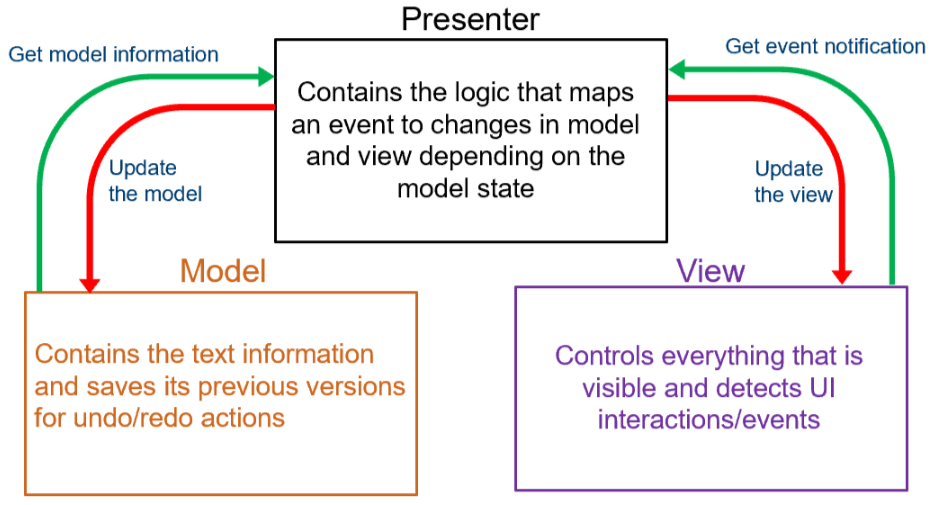
\includegraphics[scale=0.9]{mvp_diagram}
	\caption{The diagram of the Model-View-Presenter pattern}
	\label{mvp}
\end{figure*}

\vspace{-0.3cm}
\subsection{Simple gesture implementation}

Once the text editor component was finished, the work moved on to gestures. LeapMotion hand sensors are used for hand tracking. Two simple hand gestures were implemented using the LeapMotion extended finger detection and Unity colliders. Spherical colliders are placed on the tips of the fingers and a trigger is placed as a thin box around the plane.

The first gesture is the touch of the plane that places the text cursor. This was implemented by detecting when the index finger is extended and locating where the index finger collider enters the trigger of the plane.

The second implemented gesture is used to select the text. The selection is done by touching the plane with extended index and middle fingers to choose the starting point, moving the fingers parallel to the plane to choose the end point, and moving fingers away from the plane to confirm the selection. The touch and exit detection is done using the colliders on the fingers. To avoid accidental selection confirmations, the trigger area is increased after the starting point is chosen. However, because of the perspective view and the increased distance between the plane and the finger, this decreases the accuracy of the end point location. Better gestures will be explored in the gesture elicitation stage.

\vspace{-0.3cm}
\subsection{Testing}

The text editor component has been thoroughly tested using a combination of automatic unit tests and both scripted and unscripted manual tests. 66 unit tests have been written that quite extensively cover the model and the coordinate conversions in the presenter. The rest of the text editor was tested manually because of the need for visual verification. 24 manual test cases that cover most of the editor functionality have been described in a text document. Improvised testing has been done as well to check if nothing has been missed.

Unit tests are run via Unity Test Runner every time there is a text editor code change. Manual testing is done only if there is a significant code change or if there is any reason to believe that the behaviour has changed.

The system has also been tested once with the Oculus Rift HMD. The single and two finger interactions worked as expected. The potential for arm fatigue from these interactions was noted, since part of the interaction is touching the plane with the text, which might be quite large. Furthermore, the visual quality of the text was not good but the main reason seems to be the limitation of the technology used rather than the text editor itself.

% --------- FUTURE
\section{Future work}

The plan for Lent and Easter terms is shown in Figure \ref{gantt}.
\begin{figure*}
	\centering
	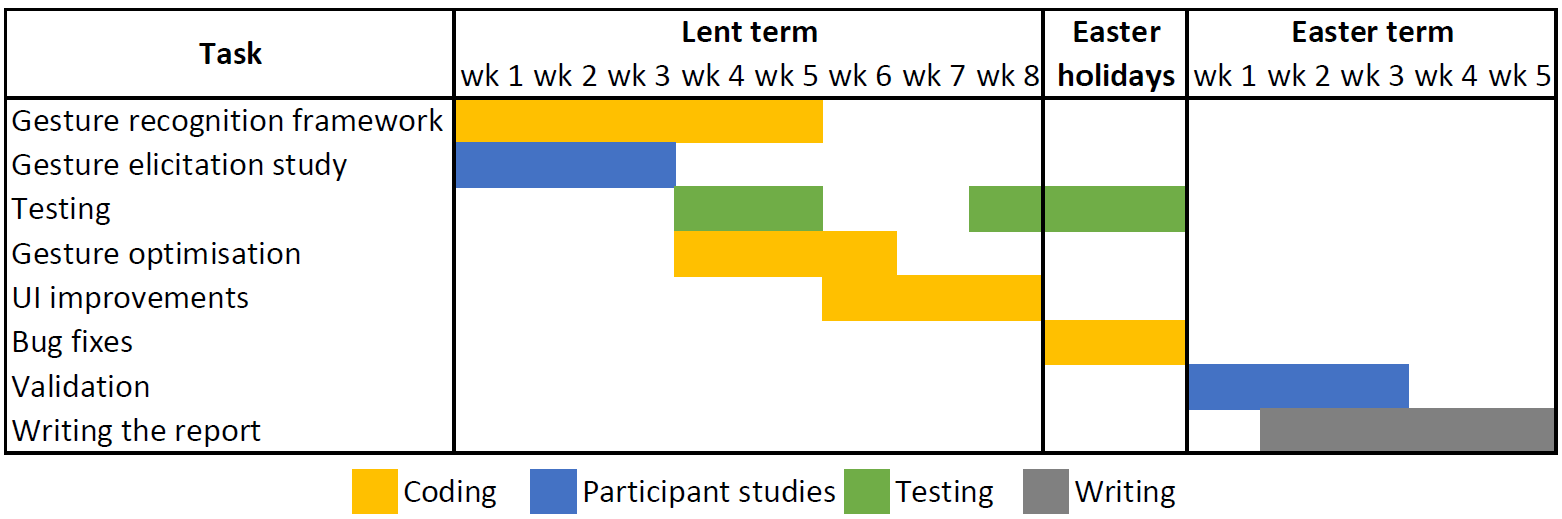
\includegraphics[scale=0.75]{gantt_chart}
	\caption{Gantt chart illustrating the plan for Lent and Easter terms}
	\label{gantt}
\end{figure*}

\vspace{-0.3cm}
\subsection{Framework for gesture recognition}
The immediate next step of the project is to build the framework for gesture recognition. Long Short-Term Memory (LSTM) neural network was chosen for the framework because of its capabilities to do gesture recognition in real time on a low power device \cite{lstm_real_time}. The representation for the input data will use an existing feature set HIF3D \cite{features} and the Temporal Pyramid feature extraction technique. The dataset that will be used during the development of the framework is the LMDHG \cite{gesture_dataset} with 608 gesture instances. For the actual gesture recognition the dataset of designed gestures will be collected in the lab. The LMDHG is quite small and the collected dataset is likely to be of a similar size, therefore, if LSTM will not perform well due to the size of the datasets, SVM will be implemented and used instead. Unit tests will be written for the framework and the model will be tested by obtaining the confusion matrices.

\vspace{-0.3cm}
\subsection{Designing gestures}
To design gestures that require minimal learning, a gesture elicitation study will be performed. Since there is a strong connection between the learning time and the guessability, the study will follow the guessibility maximisation methodology \cite{guessability}. Participants will be asked to come up with a unique gesture for each of the five actions that do not yet have a gesture assigned (see Table \ref{actions}) as well as an improved gesture for text selection. Participants will also be asked to think about the efficiency of the gesture before suggesting it. Once all the gesture suggestions are collected, a scoring function will determine which gestures are selected for the final design.

\vspace{-0.3cm}
\subsection{Optimisation of the gestures}
Optimisation of the selected gestures will be done to make the gestures as efficient as they can be, and to obtain the best possible confusion matrix results. The effects of the gesture speed, the size of the finger movements, the distance of the hand movement and the stretch of the arm will be analysed. A dataset of gestures with variations will have to be collected for this analysis. The optimisation will be done in relation to the gesture recognition framework and will involve fine-tuning the parameters to improve detectability and reduce the confusion. The cursor placement and text selection gestures (Table \ref{actions}) will be optimised as well.

\vspace{-0.3cm}
\subsection{User experience improvements}
Improving the user interface is important for overall system usability and adding visual feedback for gesture recognition can have significant effects on correct gesture recognition rates \cite{feedback}. Visual tutorials, hints and feedback will be added to the system in hopes to make it more efficient and to lower the required learning time.

\vspace{-0.3cm}
\subsection{Verification}
Testing will be a part of all the stages described before. Unit tests will be written where possible and more manual tests will be added. Already existing tests will also be run periodically to make sure that everything still works as expected.

The system will also be tested with the HMD. Ideally the LeapMotion sensor would connect to the HoloLens and the full system would be a Mixed Reality Annotation System. However, the current connection between the LeapMotion and the HoloLens is too slow and the system might be used with the Oculus Rift instead, resulting in a Virtual Reality Annotation System.

\vspace{-0.3cm}
\subsection{Validation}
If time allows, there will be an attempt to validate the system. A group of participants will be asked to perform a set of tasks and then fill in a questionnaire about their experience. However, the tests with real users are very time consuming and it is very unlikely that there will be enough time for this.

% --------- REFERENCES
\bibliographystyle{ieeetr}
\bibliography{references}

\end{document}